% \paragraph{Forward diffusion process}\mbox{} \\
% \begin{equation}
%     q(\mathbf{x}_{t}|\mathbf{x}_0)=\mathcal{N}(\mathbf{x}_{t};\sqrt{\bar{\alpha}_{t}}\mathbf{x}_0,(1-\bar{\alpha}_{t})\mathbf{I})
% \end{equation}

% \begin{equation}
% \mathbf{x}_{t}=\sqrt{\alpha_{t}}\mathbf{x}_{t-1}+\sqrt{1-\alpha_{t}}\boldsymbol{\epsilon},\quad\boldsymbol{\epsilon}\sim\mathcal{N}(0,\mathbf{I}).
% \end{equation}

% \begin{aligned}
% \mathbf{x}_t 
% &= \sqrt{\alpha_t}\mathbf{x}_{t-1} + \sqrt{1 - \alpha_t}\boldsymbol{\epsilon}_{t-1} & \text{ ;where } \boldsymbol{\epsilon}_{t-1}, \boldsymbol{\epsilon}_{t-2}, \dots \sim \mathcal{N}(\mathbf{0}, \mathbf{I}) \\
% &= \sqrt{\alpha_t \alpha_{t-1}} \mathbf{x}_{t-2} + \sqrt{1 - \alpha_t \alpha_{t-1}} \bar{\boldsymbol{\epsilon}}_{t-2} & \text{ ;where } \bar{\boldsymbol{\epsilon}}_{t-2} \text{ merges two Gaussians (*).} \\
% &= \dots \\
% &= \sqrt{\bar{\alpha}_t}\mathbf{x}_0 + \sqrt{1 - \bar{\alpha}_t}\boldsymbol{\epsilon} \\
% q(\mathbf{x}_t \vert \mathbf{x}_0) &= \mathcal{N}(\mathbf{x}_t; \sqrt{\bar{\alpha}_t} \mathbf{x}_0, (1 - \bar{\alpha}_t)\mathbf{I})
% \end{aligned}

\begin{figure}[h]
    \centering
    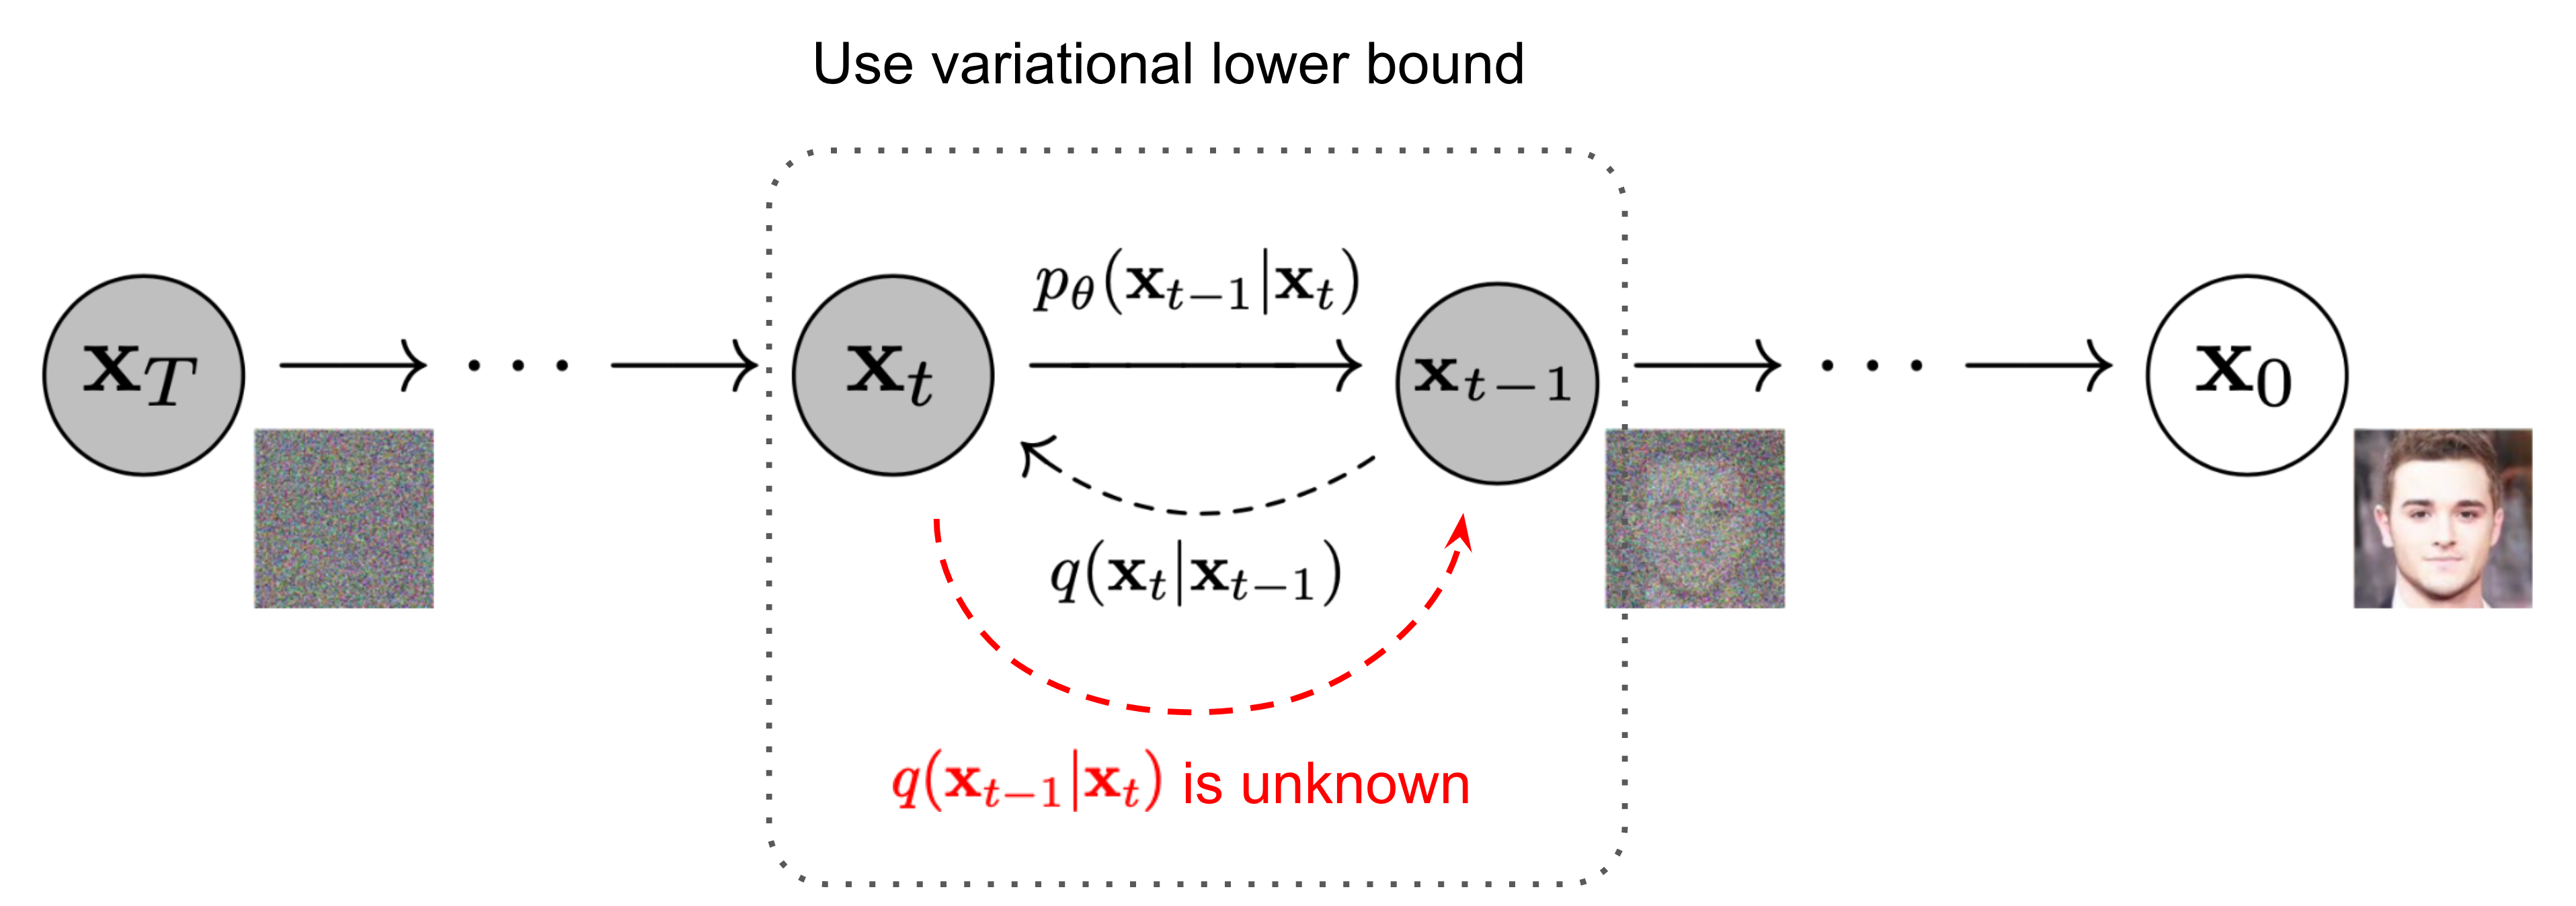
\includegraphics[width=0.9\linewidth]{concept_engineering/ddpm/DDPM.png}
    \caption{Visualization of the diffusion process\cite{ho2020denoisingdiffusionprobabilisticmodels}.}
    \label{fig:diffusion-process}
\end{figure}
Denoising Diffusion Probabilistic Models (DDPM)\cite{ho2020denoisingdiffusionprobabilisticmodels} are generative models that work by gradually adding noise to the data in several steps, and then learning how to reverse this process to recover the original data. The model learns to denoise the image step by step, starting from pure noise and progressively improving its reconstruction until it produces a realistic image. This approach allows DDPM to produce highly detailed synthetic images. 


\paragraph{Loss function}\mbox{}\\
\indent The loss function in DDPM is based on the evidence lower bound (ELBO\footnote{\url{https://en.wikipedia.org/wiki/Evidence_lower_bound}}), also known as "variational lower bound", which involves minimising the difference between the data distribution and the model distribution at each step of the diffusion process. In particular, it includes a term that encourages the model to effectively learn the backward diffusion process.

In practice, ELBO optimization is only the theoretical objective in DDPMs.
\textbf{M}ean \textbf{S}quared \textbf{E}rror and sometimes \textbf{A}bsolute \textbf{E}rror are the practical ways of loss calculation. They are used to calculate an error between added noise and predicted noise. The training objective is to minimize this error. This approach is an approximation of the ELBO optimization.\footnote{Full derivation can be seen in \cite{ho2020denoisingdiffusionprobabilisticmodels} or in this blogpost \url{https://learnopencv.com/denoising-diffusion-probabilistic-models/}}. 

% \begin{equation}
%     \centering
%     L(\theta)=\mathbb{E}_{t, x_0, \epsilon}\left[\left\|\epsilon-\epsilon_\theta\left(x_t, t\right)\right\|^2\right]
%     \label{loss-ddpm}
% \end{equation}

\begin{equation}
\begin{aligned} L_{\text {simple }}(\theta) & :=E_{t \sim U[1, T], \mathbf{x}_0, \epsilon}\left[\left\|\epsilon-\epsilon_\theta\left(\mathbf{x}_t, t\right)\right\|^2\right] \\ & =E_{t \sim U[1, T], \mathbf{x}_0, \epsilon}\left[\left\|\epsilon-\epsilon_\theta\left(\sqrt{\bar{\alpha}_t} \mathbf{x}_0+\sqrt{1-\bar{\alpha}_t} \epsilon, t\right)\right\|^2\right],
\end{aligned}
\end{equation}

where:
\begin{itemize}
    \item $x_0$ - original image,
    \item $T$ - number of timesteps, usually hundreds,
    \item $t$ - particular timestep,
    \item $\epsilon$ - gaussian noise added to original image,
    \item $\theta$ - neural network, for example U-Net,
    \item $\epsilon_\theta(x_t, t)$ - noise predicted by a neural network for a timestep $t$,
    \item $\overline{\alpha_t}$ - scaling factor.
\end{itemize}

The scaling factor is defined as cumulative product of all $\alpha$ between 1 and $t$:
\begin{equation}
    \overline{\alpha_t} = \prod_{s=1}^t \alpha_s,
\end{equation}

and 
\begin{equation}
    \alpha_t = 1-\beta_t.
\end{equation}

The term $\beta_t$ is called "diffusion rate" for timestep $t$ and is calculated using a "noise scheduler". Such scheduler controls how much noise is added to an image in each step. Noise scheduler can be, for example, linear, scaled linear or squared cosine cap.

\paragraph{Training process}\mbox{}\\

\begin{figure}[H]
    \centering
    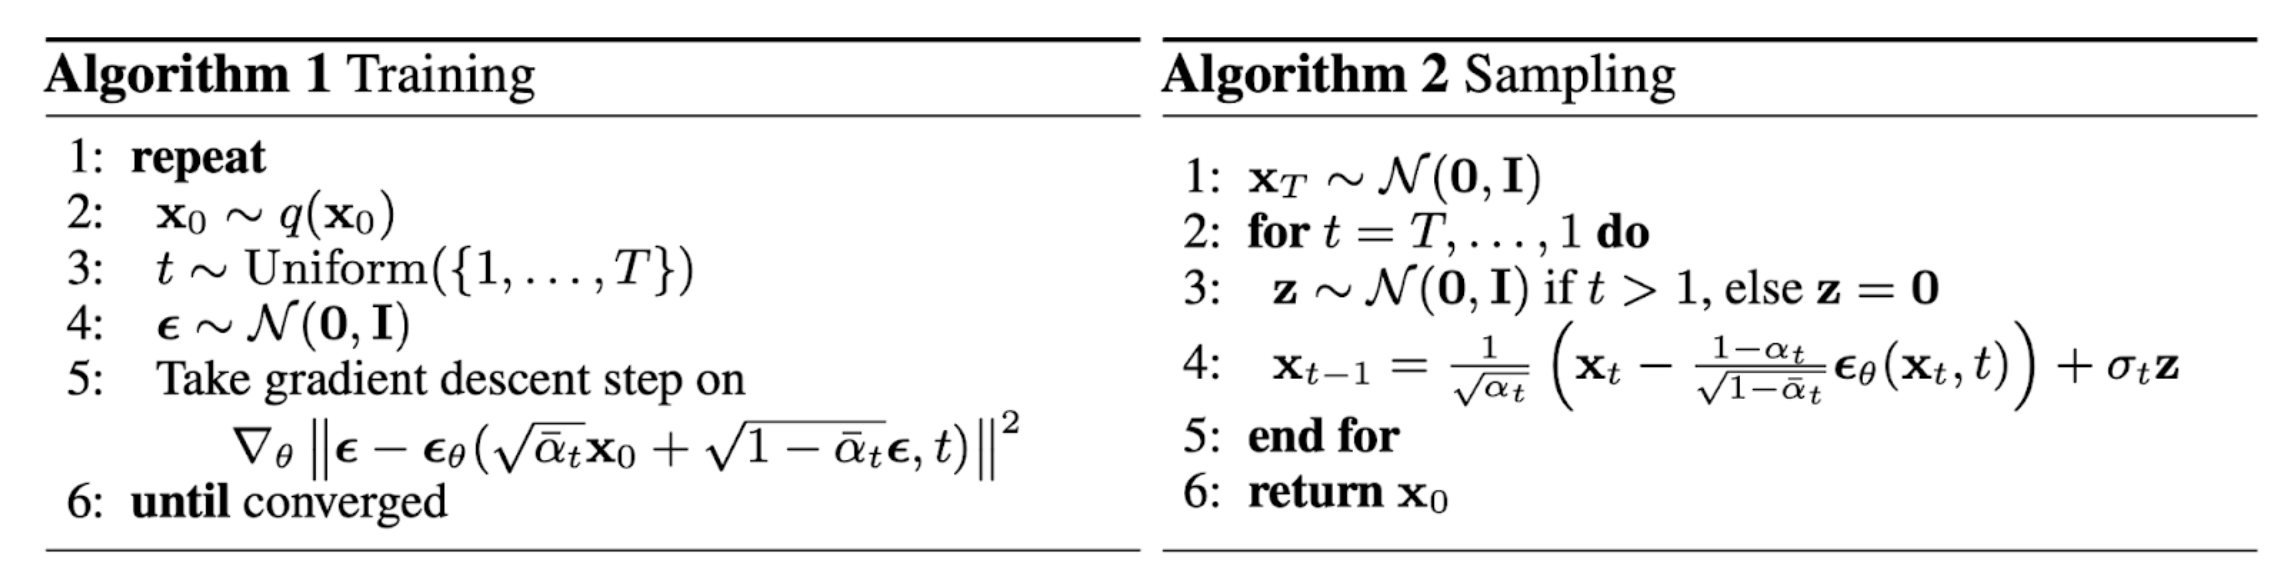
\includegraphics[width=0.9\linewidth]{concept_engineering/ddpm/DDPM-algo.png}
    \caption{Training and sampling algorithms for the diffusion process\cite{ho2020denoisingdiffusionprobabilisticmodels}.}
    \label{fig:diffusion-algo}
\end{figure}
In the training algorithm[\ref{fig:diffusion-algo}] the loss is calculated as a squared error between noise and predicted noise at a timestep $t$. However in practice all squared errors are calculated for each timestep $t$ and then final loss over an image (or a scan in 3D case) is calculated as a mean of these squared errors - MSE. 
This final loss is then aggregated with losses from the whole batch. At this point the gradient is calculated.  

\paragraph{Generation of CT scans}\mbox{}\\
\indent To generate artificial CT scans using DDPM, we could start by sampling gaussian noise and iteratively apply the learned reverse diffusion process. This process should refine the noise into a synthetic CT image that would progressively capture more and more of the anatomical details of the pelvis region.


\paragraph{Latent Diffusion Models}\mbox{}\\
\indent Latent diffusion models are diffusion models but in the latent space of an autoencoder. Unlike original diffusion, they do not generate an image from a Gaussian noise, but they generate its latent representation from a Gaussian noise. Then we can use a decoder to generate an image.
% \begin{figure}
%     \centering
%     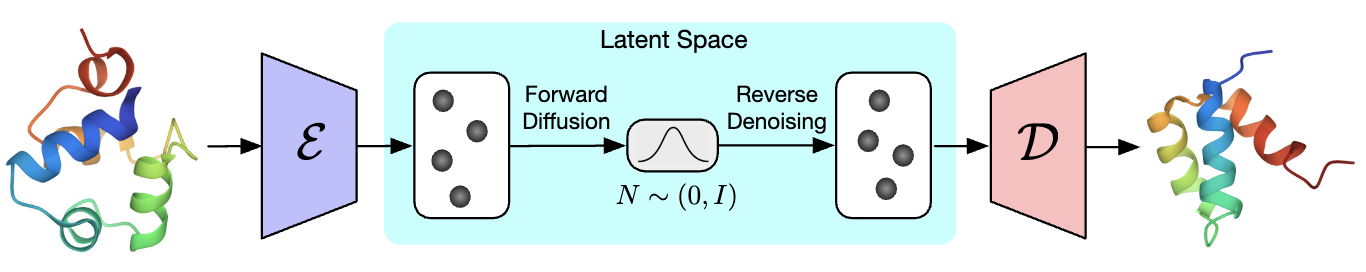
\includegraphics[width=\linewidth]{concept_engineering/ldm/LatentDiff.png}
%     \caption{Caption}
%     \label{fig:enter-label}
% \end{figure}

\begin{figure}[H]
    \centering
    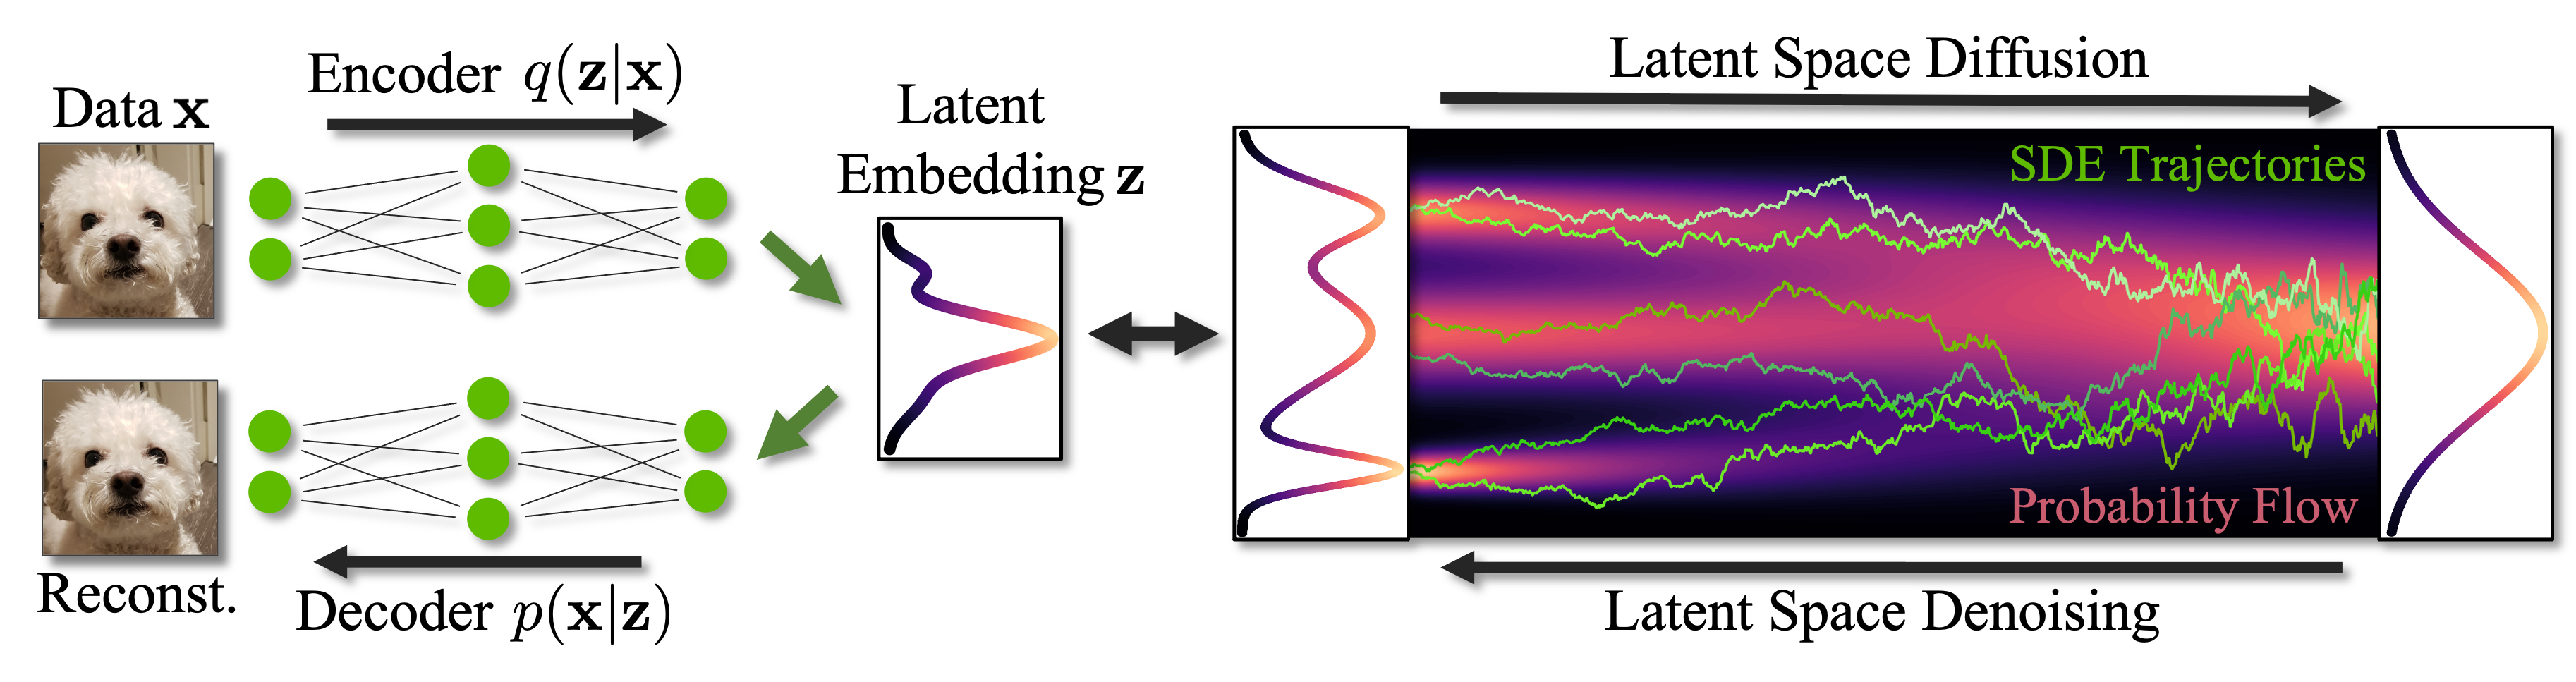
\includegraphics[width=\linewidth]{concept_engineering/ldm/ldm_figure.png}
    \caption{Visualization on how Latent Diffusion Models work. LDM learns latent representations distribution instead of distribution of input data\cite{neurips2023-ldm-tutorial/neurips2023-ldm-tutorial.github.io_2023}.}
    \label{fig:ldm}
\end{figure}

The idea of using diffusion model in the latent space will be used in the architectures below.
More information on LDM can be found on the website\footnote{\url{https://neurips2023-ldm-tutorial.github.io/}} and in the presentation\footnote{\url{https://drive.google.com/file/d/1p_aZ627Bwvku7nKyYRHtfZe50nAnpqGU/view}}.
